% Online sync refresh: revised workshop report, 2026-08-29. figure-path-fix
To investigate the sensitivity of the gradient-bandit algorithm to the
learning rate, the experiment was repeated for
\[
    \alpha\in
    \{0.01,\,0.05,\,0.1,\,0.5,\,1,\,2,\,5\}.
\]
For each value of $\alpha$, the algorithm was run over $T=10^4$ time steps
and $M=300$ independent reruns. At each time step, the probability assigned
by the softmax policy to the true optimal arm
\[
    a^\ast\in\arg\max_{a\in\mathcal A}q^\ast(a)
\]
was recorded and averaged across reruns. Thus, convergence to the optimal
decision corresponds to the mean probability of selecting $a^\ast$
approaching one.

\begin{figure}[H]
    \centering
    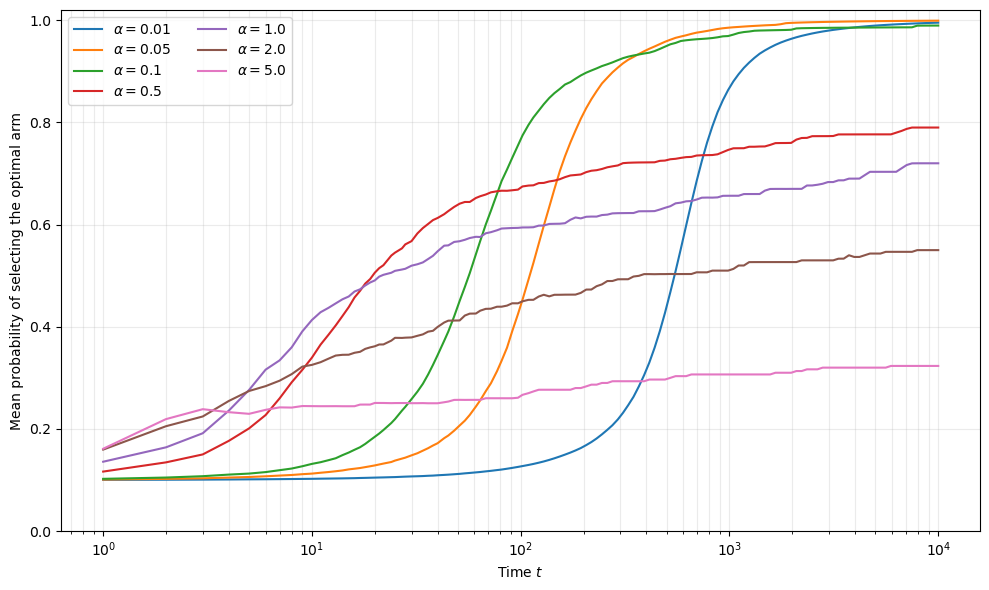
\includegraphics[width=0.92\linewidth]
    {figures/q7_gradient_alpha_sensitivity.png}
    \caption{Mean probability of selecting the optimal arm for different
    gradient-bandit learning rates.}
    \label{fig:q7-gradient-alpha}
\end{figure}

Figure~\ref{fig:q7-gradient-alpha} shows that satisfactory finite-horizon
concentration on the optimal arm is not obtained for every tested
$\alpha>0$. For the smaller learning rates
$\alpha=0.01$, $0.05$, and $0.1$, the probability of selecting the optimal
arm approaches approximately one by the end of the simulation. However,
performance deteriorates as the learning rate becomes large. At
$T=10^4$, the optimal-arm probabilities are only approximately $0.79$,
$0.72$, $0.55$, and $0.33$ for
$\alpha=0.5$, $1$, $2$, and $5$, respectively.

The mean curves hide a strongly bimodal run-level outcome. The final
probabilities are summarised in Table~\ref{tab:q7-concentration}.

\begin{table}[H]
    \centering
    \caption{Run-level concentration of the final optimal-arm probability
    $P_T(a^\ast)$ over $300$ reruns.}
    \label{tab:q7-concentration}
    \begin{tabular}{ccccc}
        \toprule
        $\alpha$ & Mean $P_T(a^\ast)$ & $P_T(a^\ast)>0.99$
        & $P_T(a^\ast)<0.01$ & Between \\
        \midrule
        $0.01$ & $0.9952$ & $1.0000$ & $0.0000$ & $0.0000$ \\
        $0.05$ & $0.9991$ & $1.0000$ & $0.0000$ & $0.0000$ \\
        $0.10$ & $0.9896$ & $0.9900$ & $0.0100$ & $0.0000$ \\
        $0.50$ & $0.7899$ & $0.7900$ & $0.2100$ & $0.0000$ \\
        $1.00$ & $0.7200$ & $0.7200$ & $0.2800$ & $0.0000$ \\
        $2.00$ & $0.5500$ & $0.5500$ & $0.4500$ & $0.0000$ \\
        $5.00$ & $0.3233$ & $0.3233$ & $0.6767$ & $0.0000$ \\
        \bottomrule
    \end{tabular}
\end{table}

For large $\alpha$, most reruns therefore assign either more than $0.99$ or
less than $0.01$ probability to the optimal arm, rather than fluctuating
around an intermediate policy. Large learning rates produce large
stochastic preference updates and often cause premature near-deterministic
concentration. Depending on early reward observations, this concentration
may be on either the optimal arm or a suboptimal arm.

Therefore, the numerical experiment demonstrates strong learning-rate
sensitivity for this bandit instance. Smaller tested values give behaviour
consistent with concentration on the optimal arm by $T=10^4$, whereas large
values frequently concentrate on a suboptimal arm. Since the experiment has
a finite horizon, it does not by itself prove a general asymptotic
convergence or non-convergence theorem for constant-step gradient bandits.
